\section{ARDUINO}

Una buena definición de lo que es Arduino lo da la Wikipedia; <<Arduino es una plataforma de hardware libre, basada en una placa con un microcontrolador y un entorno de desarrollo, diseñada para facilitar el uso de la electrónica en proyectos multidisciplinares.>>.

\subsection{Hardware}

El hardware consiste en una placa con un microcontrolador \emph{Atmel AVR} y puertos de entrada/salida. Los microcontroladores más usados son el \emph{Atmega168}, \emph{Atmega328}, \emph{Atmega1280}, \emph{ATmega8} por su sencillez y bajo coste que permiten el desarrollo de múltiples diseños.

\begin{figure}[h!]
    \centering
    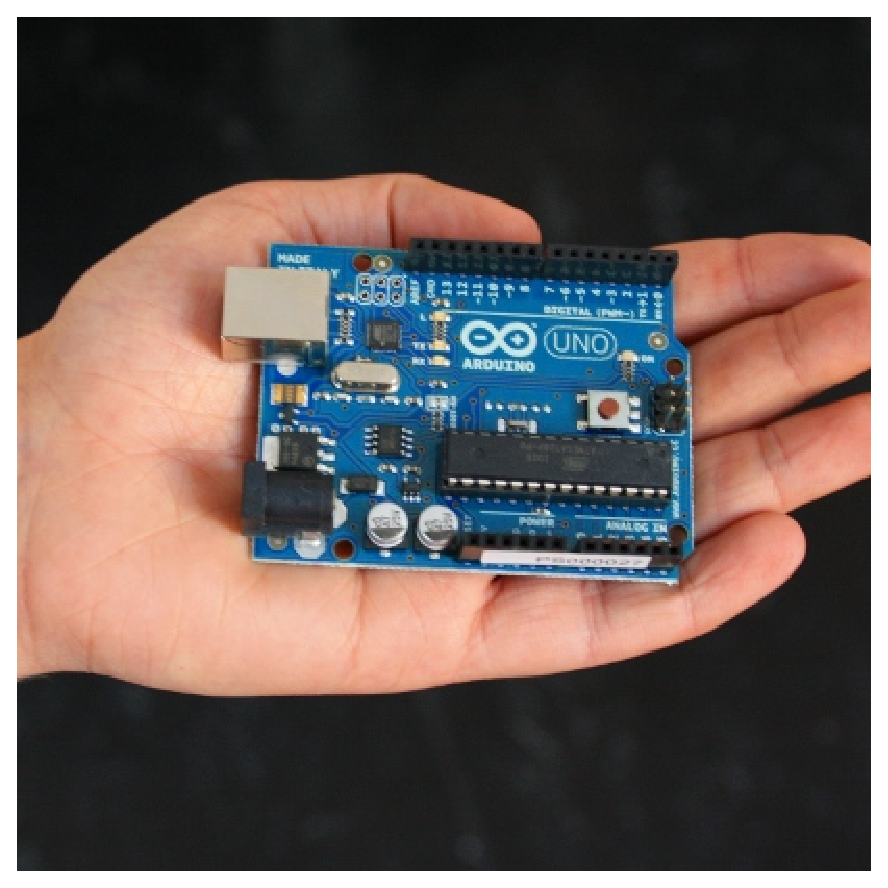
\includegraphics[keepaspectratio,width=0.6\textwidth]{arduino_uno_test.eps}
    \label{fig:arduino_uno_test}
\end{figure}


Por otro lado el software consiste en un entorno de desarrollo que implementa el lenguaje de programación \emph{Wiring} y el cargador de arranque que es ejecutado en la placa.

\begin{figure}[h!]
    \centering
    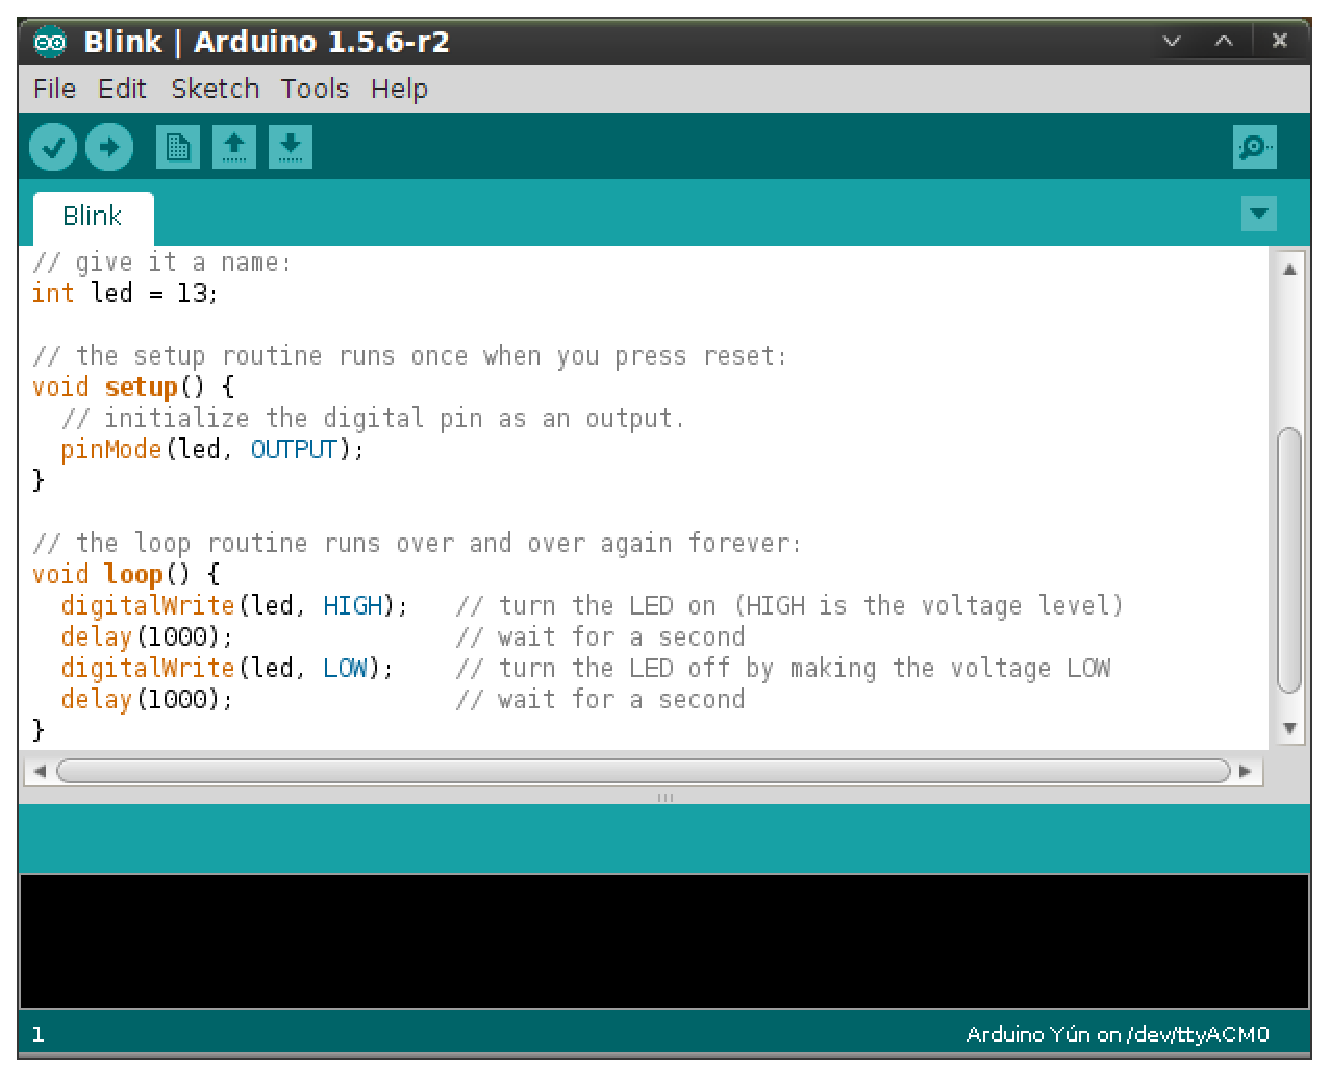
\includegraphics[keepaspectratio,width=0.6\textwidth]{arduino-ide.eps}
    \label{fig:arduino-ide}
\end{figure}

El lenguaje de alto nivel \emph{Wiring}, implementado en C/C++, permite una programación sencilla del hardware. Comparte todas las funciones estándar de C, algunas de C++ y añade las propias para el manejo de puertos (digitales, analógicos).

A continuación se muestra un código sencillo para hacer parpadear un diodo led cada segundo, se utiliza el puerto 8 digital de la placa \emph{Arduino}:

\begin{lstlisting}
    void setup() {
      pinMode(8, OUTPUT);
    }

    boolean encendido = false;
    void loop() {
      if(!encendido) {
        digitalWrite(8, HIGH);
      } else {
        digitalWrite(8, LOW);
      }
      encendido!=encendido;
      delay(1000);
    }
\end{lstlisting}


\subsection{Proyectos}